\psfrag{an}[c][c] {$\text{\scriptsize Solid anode}$}
\psfrag{ca}[c][c] {$\text{\scriptsize Solid cathode}$}
\psfrag{fd}[c][c] {$\text{All-solid-state battery}$}
\psfrag{ch}[c][c] {$\text{Sample: IEK - FZ Jülich}$}

\psfrag{xx}[l][l] {$\text{Li}+$}
\psfrag{xxx}[l][l] {$\text{Lithium Lanthanum Zirconate}$}
\psfrag{em}[l][l] {$\text{e}-$}
\psfrag{sele}[c][c] {$\text{\scriptsize Solid electrolyte}$}
\psfrag{gr}[l][l] {$\text{Lithium metal}$}
\psfrag{mo}[l][l] {$\text{Metal-oxide}$}
\psfrag{xma}[l][l] {$\text{La}_{7}\text{Li}_{3}\text{Zr}_{2}\text{O}_{12}$}

\psfrag{xbf}[l][l] {$\text{\scriptsize  No electric field}$}
\psfrag{xat}[l][l] {$\text{\scriptsize  Under electric field}$}

\psfrag{mic}[l][l] {$\text{Microscale: Part 2}$}
\psfrag{mac}[l][l] {$\text{Macroscale: Part 1}$}
\psfrag{sca}[c][c] {$\text{Scale}$}
\psfrag{xgr}[c][c] {$\text{\scriptsize Grains}$}
\psfrag{xgrb}[c][c] {$\text{\scriptsize Grain boundaries}$}
\psfrag{gbb}[c][c] {$(\star)\ \text{\scriptsize Grain boundary}$}
\psfrag{st}[l][l] {$(\star)$}
\psfrag{g1}[c][c] {\small $\text{Grain 1}$}
\psfrag{g2}[c][c] {\small $\text{Grain 2}$}

\psfrag{xm}[c][c] {$-$}
\psfrag{xp}[c][c] {$+$}
\psfrag{dta}[c][c] {$\delta$}

\psfrag{a}[c][c] {$\text{\faBolt}$}
\psfrag{F}[c][c] {$\text{F}$}

\psfrag{sse}[c][c] {$\text{Solid-state electrolyte}$}

\psfrag{masca}[c][c] {$\text{Macroscale}$}
\psfrag{mesca}[c][c] {$\text{Mesoscale}$}
\psfrag{misca}[c][c] {$\text{Microscale}$}

%--------------------------------------------------------

\psfrag{seleb}[c][c] {\small $\text{\scriptsize Misorientation}$}
\psfrag{selec}[c][c] {\small $\text{\scriptsize Multi-preferred directions}$}

\psfrag{dispmu}[c][c] {\small $\textsc{displacement field } \Bu$}
\psfrag{pbar}[c][c] {\small$\Bu=\bar{\Bu}$}
\psfrag{dbt}[c][c] {\small$\partial\Omega^{\Bt}_{N}$}
\psfrag{dbphi}[c][c] {\small$\partial\Omega^{\Bu}_{D}$}
%\psfrag{n}[c][c] {$\Bn$}
\psfrag{n}[c][c] {\small $\Bn$}
%\psfrag{tbar}[c][c] {$\Bt:=\Bsigma\cdot\Bn$}
\psfrag{tbar}[c][c] {\small $\Bsigma\cdot\Bn = \bar{\Bt}$}
\psfrag{phi}[c][c] {\small $\Bu$}


\psfrag{concen}[c][c] {\small $\textsc{structure tensor } \BM^{R} \circ \BM^{E}$}
%\psfrag{cbar}[c][c] {$c=\bar{c}$}
\psfrag{cbar}[c][c] {\small $\phi=\bar{\phi}$}
\psfrag{dbh}[c][c] {\small $\partial\Omega^{h}_{N}$}
\psfrag{dbc}[c][c] {\small $\partial\Omega^{\phi}$}
%\psfrag{n}[c][c] {$\Bn$}
%\psfrag{hbar}[c][r] {$h := \KIh\cdot\Bn$}
%\psfrag{hbar}[c][r] {$\KIH\cdot\Bn = \bar{H}$}

\psfrag{c1}[c][c] {\small $\Bd^{R}_{G_1}$}
\psfrag{c2}[c][c] {\small $\Bd^{R}_{G_2}$}

\psfrag{gd1}[l][l] {\small $\text{Grain-1}$}
\psfrag{gd1p}[l][l] {\small $\text{preferred}$}
\psfrag{gd1d}[l][l] {\small $\text{direction}$}

\psfrag{gd2}[c][c] {\small$\text{Grain-2}$}
\psfrag{gd2p}[c][c] {\small$\text{preferred}$}
\psfrag{gd2d}[c][c] {\small$\text{direction}$}

\psfrag{ce}[c][c] {\small $\Bd^{E}$}

\psfrag{rsbulk}[c][c] {\small $\text{rest of the bulk}$}
\psfrag{mu}[c][c] {\small $\phi$}

\psfrag{xb}[c][c] {\small $\Bx \in \Omega$}

\psfrag{str}[c][c] {\small $\BM^{R} := \Bd^{R} \otimes \Bd^{R}$}
\psfrag{mde}[c][c] {\small $\BM^{E} := \Bd^{E} \otimes \Bd^{E}$}

\psfrag{cp}[c][c] {\small $\text{preferred direction}$}

\psfrag{temp}[c][c] {\small $\textsc{temperature field } \theta$}
\psfrag{te}[c][c] {\small $\theta$}
\psfrag{tebar}[c][c] {\small $\theta = \bar{\theta}$}
\psfrag{dbte}[c][c] {\small $\partial\Omega^{\theta}_{D}$}
\psfrag{hbar}[c][c] {\small $\Bq\cdot\Bn = \bar{h}$}

\psfrag{ecpu}[l][l] {\small $\text{Uniform}$}
\psfrag{ecpep}[l][l] {\small $\text{electric-potential}$}
% \psfrag{ecpid}[l][l] {$\text{induced direction}$}
\psfrag{ecpid}[l][l] {\small $\text{polarizational effect}$}

\psfrag{pl}[l][l] {\small $+$}
\psfrag{mn}[l][l] {\small $-$}

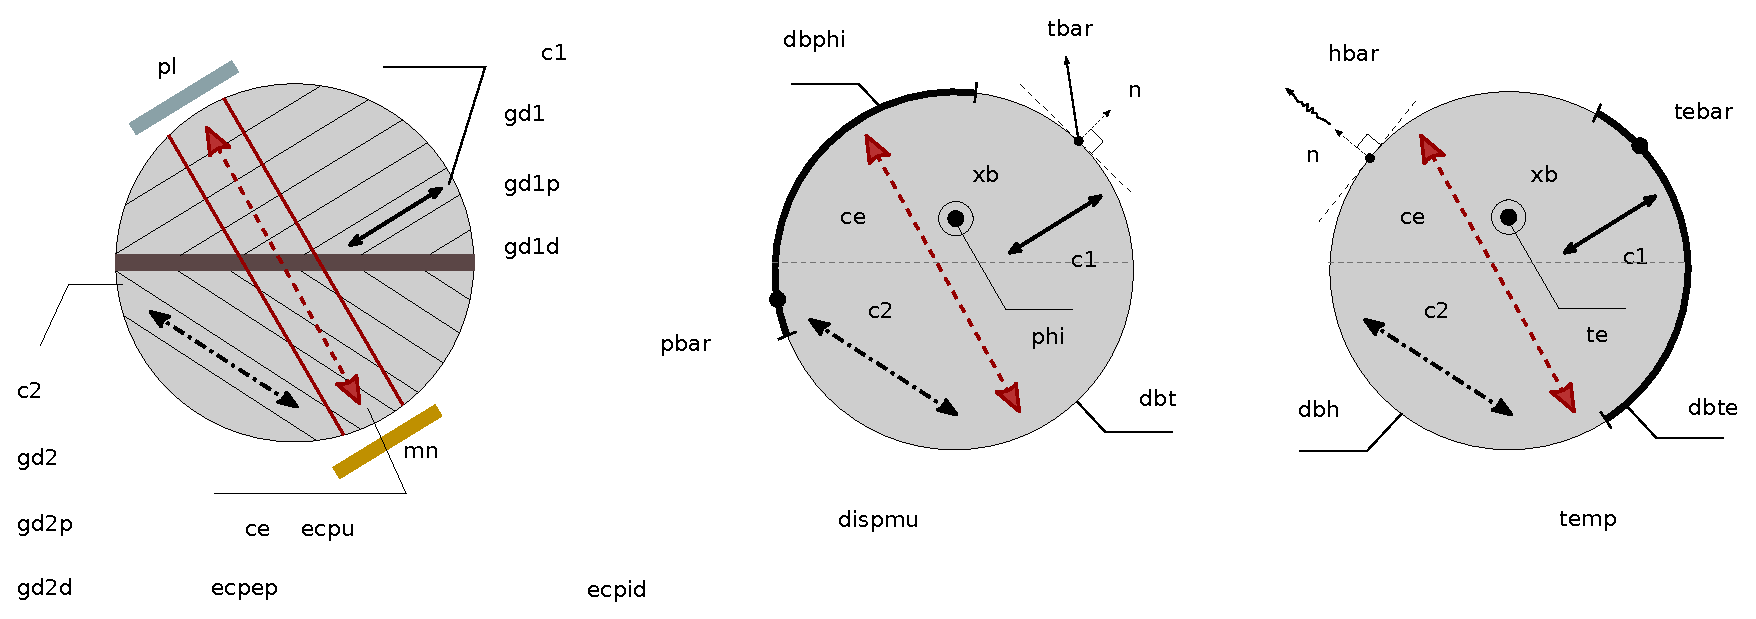
\includegraphics[width=0.75\textwidth]{structuraltwofields.eps}
% \caption{Multi-structural internal variables $\Bd^{R}_{G_{i},i=1,\dots,N}$
% as referential material direction of $N^{th}$ grains, 
% and $\Bd^{E}$ as the globally uniform electric-potential direction,
% and the two governing fields: displacement $\Bu$ and temperature $\theta$.
% Dirichlet and Neumann boundary conditions are $\partial\Omega_{D}$ 
% and $\partial\Omega_{N}$, respectively.}